\documentclass{article}
\usepackage[margin=1.5cm,bottom=2cm]{geometry}
\usepackage{fancyhdr}
\usepackage{graphicx}
\usepackage{amsmath}
\pagestyle{fancy}

\begin{document}
\fancyhead[L]{ 
\includegraphics[width=2cm]{au_logo.png} }
\fancyhead[R]{PHYS 4220: Computational Physics}
\fancyfoot[C]{\thepage}
\vspace*{0cm}
\begin{center}
	{\LARGE \textbf{Homework 1}}\\
	\vspace{0.25cm}
	{\Large Due: Friday, September 18}
\end{center}

\newcommand{\textbook}{\textit{Giordano}}
\begin{enumerate}
\item Consider the differential equation describing a freely falling object near the surface of the Earth:
\begin{equation*}
	\frac{dv}{dt}=-g
\end{equation*}
You may use any initial condition for $v(t=0)$ that you like. Solve for $v(t)$ both analytically and numerically (using the Euler method). Plot both solutions. Do this for several different values of the time step $\Delta t$. How does varying the time step affect the accuracy of your numerical solution? Explain your observations.
\item Consider the differential equation for an object's velocity in the presence of both a constant acceleration and frictional force:
\begin{equation*}
\frac{dv}{dt}=a-bv
\end{equation*} 
here $a$ and $b$ are constants. $a$ represents a constant applied force, such as gravity or a uniform electric field. A frictional term arises which is proportional to $v$, with $b$ as the constant of proportionality ($b>0$). Thus $b=0$ corresponds to a vacuum; increasing $b$ essentially corresponds to increasing density of the medium. This term is negative, as the force of friction opposes the direction of motion.
	\begin{enumerate}
		\item What are the dimensions of $a$ and $b$?
		Example: In class we found the dimensions of the spring constant $k$: 
		$[k]=\frac{[F]}{L}=\frac{ML}{T^2}\frac{1}{L}=\frac{M}{T^2}$; $M=$mass, $L$=length, $T=$time.
		\item By changing the units of $v$ and $t$, normalize this equation (make it dimensionless). You should be able to arrive at an equation which is independent of $a$ and $b$.
		\item Solve the dimensionless equation both analytically and numerically. Plot the solutions. Explore the behavior of the system for different initial velocities. There are three particularly interesting cases to be examined.
		\item In every case explored above, the velocity asymptotically approaches the same value. What value is it? What is this in physical units (in terms of $a$ and $b$)? Briefly comment on the physical significance of this result.
	\end{enumerate}
\item\label{decay} The long-term behavior of radioactive decay can be described by assuming that the rate of decay of material is proportional to the amount of material remaining: $\frac{dN}{dt}\propto-N$. The constant of proportionality has dimensions of $time^{-1}$ and can be expressed as $\frac{1}{\tau}$, where $\tau$ is the time scale governing the interaction and is related to the half-life of the material. We can thus write $\frac{dN}{dt}=-\frac{1}{\tau}N$. 

Now consider the process of coupled radioactive decay involving nuclei $A$ and $B$. Starting with an initial amount of $A$ $N_{A,0}$ and $B$ $N_{B,0}$, $A$-type nuclei decay directly into $B$-type nuclei with a time scale of $\tau_A$. $B$-type nuclei, which, in addition to the initial amount $N_{B,0}$, also consist of former $A$-type nuclei which have decayed into new $B$ nuclei. This situation is illustrated in Figure \ref{fig_decay}.

\begin{figure}[ht!]
	\centering
	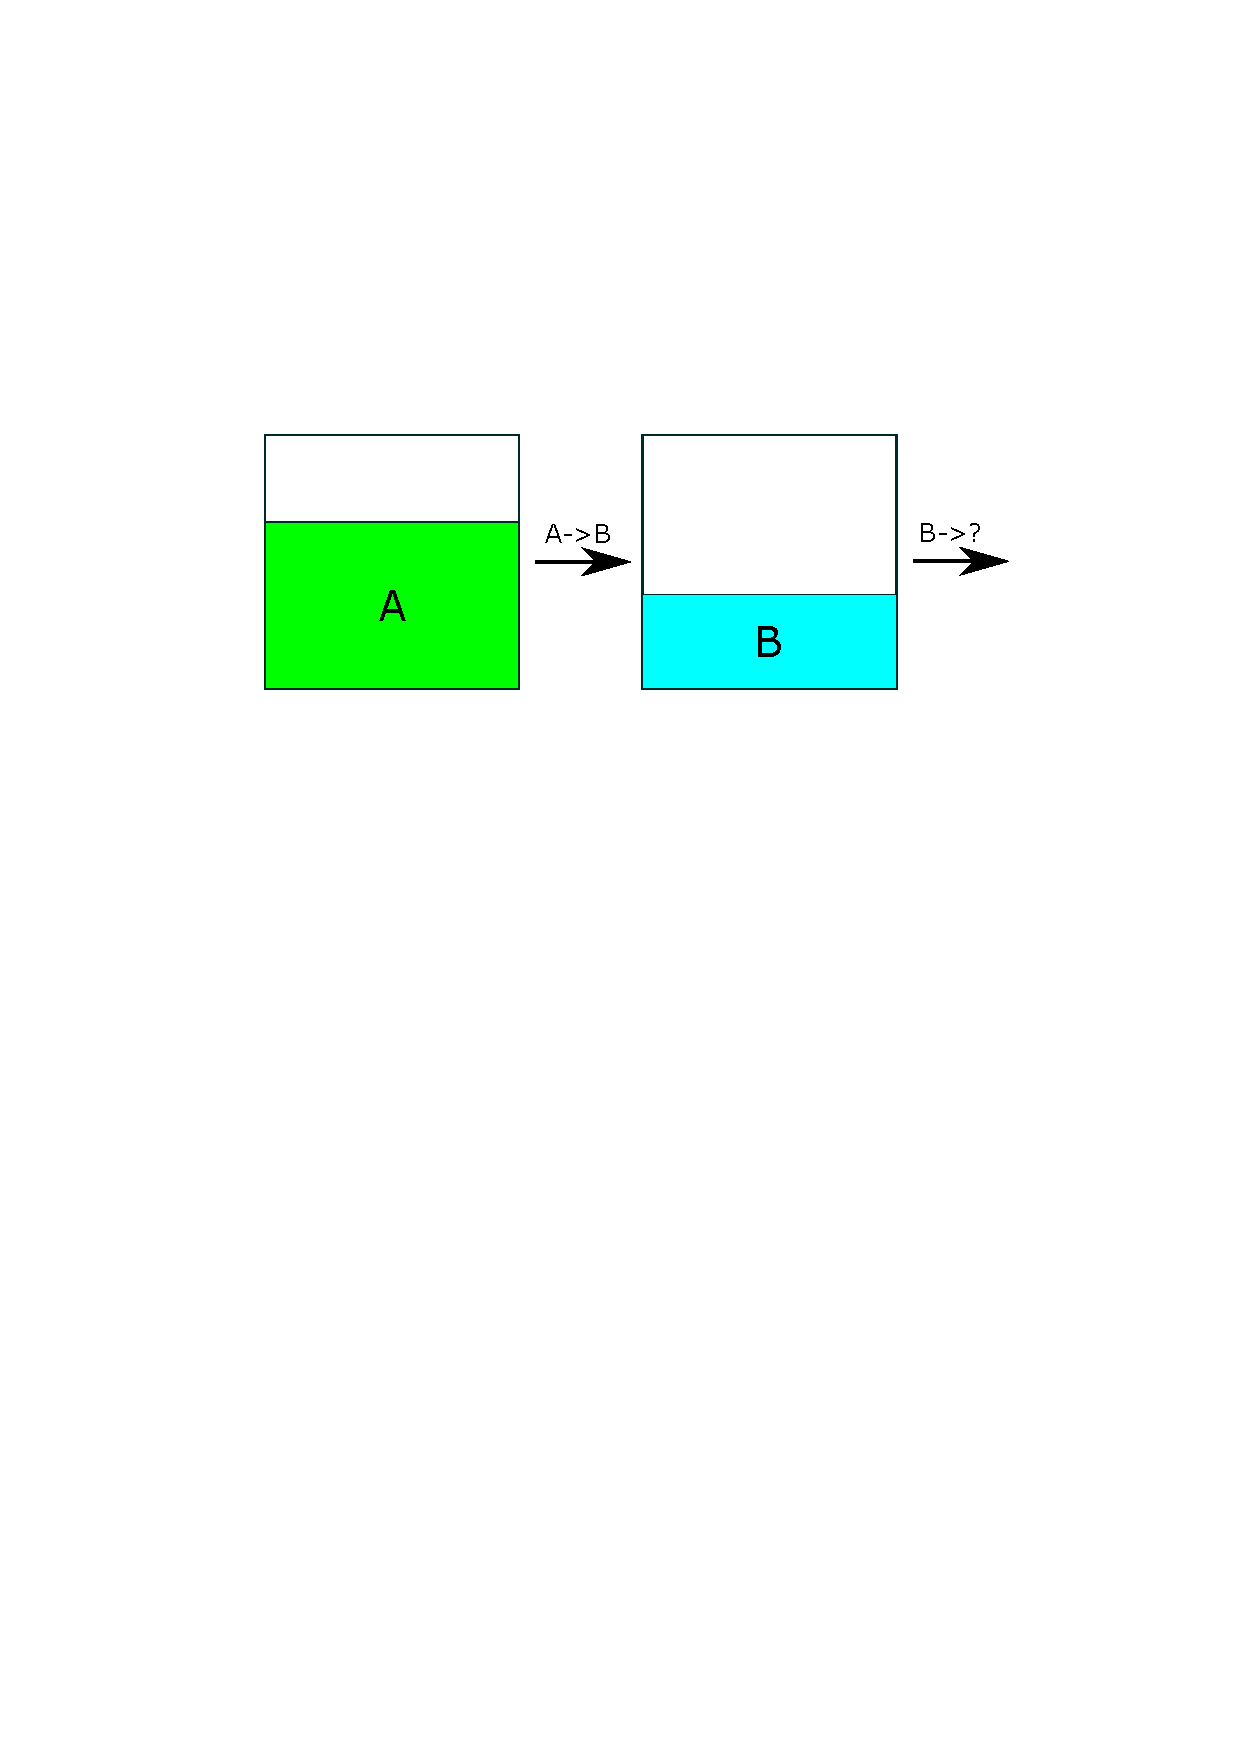
\includegraphics[width=0.5\textwidth]{drawing_hw1.pdf}
	\label{fig_decay}
	\caption{Figure for problem \ref{decay}}
\end{figure}

	\begin{enumerate}
		\item Write the differential equation governing the decay rate of $A$-type nuclei$^*$
		\item Write the differential equation governing the decay rate of $B$-type nuclei$^*$
		
		{\footnotesize $^*$ It is recommended that you verify with your instructor that your equations are correct before continuing, lest you proceed with the wrong system!}
		\item By changing the units of $N_A$, $N_B$, and $t$, rewrite this system of equations in a dimensionless form. Assume $N_{A,0}=N_{B,0}$. (\textit{Hint: $\tau_A$ or $\tau_B$ both make for a natural choice for time units. You should then find that the resulting equation depends not on either $\tau_A$ or $\tau_B$, but on the ratio of the two.})
		\item Solve this system numerically, and investigate its behavior for different values of the ratio $\tau_A/\tau_B$.
		\item \textit{Optional:} This system can be solved analytically. This can be a useful check for your numerical approximation, but is not required.
	\end{enumerate}
\end{enumerate}

\end{document}